% presentation.tex
\documentclass[aspectratio=169,11pt]{beamer}

\usepackage[utf8]{inputenc}
\usepackage[T1]{fontenc}
\usepackage{lmodern}
\usepackage{graphicx}
\usepackage{booktabs}
\usepackage{array}
\usepackage{microtype}

\graphicspath{{resources/images/}}

\usetheme{Madrid}
\usefonttheme{professionalfonts}
\setbeamertemplate{navigation symbols}{}
\setbeamertemplate{footline}[frame number]

\definecolor{AcademicBlue}{RGB}{28,65,112}
\definecolor{AcademicGray}{RGB}{82,88,96}
\setbeamercolor{structure}{fg=AcademicBlue}
\setbeamercolor{frametitle}{bg=AcademicBlue,fg=white}
\setbeamercolor{title}{fg=AcademicBlue}
\setbeamercolor{subtitle}{fg=AcademicGray}
\setbeamerfont{frametitle}{series=\bfseries,size=\large}
\setbeamerfont{itemize/enumerate body}{size=\small}
\setbeamerfont{itemize/enumerate subbody}{size=\footnotesize}
\newcommand{\nr}{n/r}

\title[Biomedical RAG Thesis]{Design and Evaluation of a Retrieval Augmented Biomedical Platform for Thrombosis Risk Factor Extraction}
\subtitle{Continuous PubMed Scheduling and Human-in-the-Loop Curation}
\author[N. Chaikalis]{Nikolaos Chaikalis}
\institute[DUTH]{School of Medicine, MSc Biomedical Informatics}
\date{June 2026}

\begin{document}

\begin{frame}
\centering
\vspace{0.35cm}
{\Large\bfseries\color{AcademicBlue}
Design and Evaluation of a Retrieval Augmented Biomedical Platform\\
for Thrombosis Risk Factor Extraction\par}

\vspace{0.35cm}
{\large\color{AcademicGray} Continuous PubMed Scheduling and Human-in-the-Loop Curation\par}

\vspace{0.85cm}
{\normalsize Nikolaos Chaikalis\par}
{\small Supervisor: Professor Eleni Kaldoudi\par}

\vspace{0.5cm}
{\small School of Medicine\\MSc Biomedical Informatics\par}

\vfill
{\small June 2026\par}
\end{frame}

\begin{frame}{Research Problem}
\begin{itemize}
  \item Biomedical evidence changes faster than static literature reviews and keyword-only search workflows.
  \item Standalone generation can produce fluent answers without inspectable evidence grounding.
  \item A biomedical question answering platform must connect freshness, semantic retrieval, provenance, and evaluation.
  \item The thesis asks how continuous ingestion, retrieval-grounded synthesis, and reproducible measurement can be unified in one architecture.
\end{itemize}
\end{frame}

\begin{frame}{Objectives}
\begin{itemize}
  \item Design a modular biomedical RAG architecture with clear acquisition, retrieval, synthesis, and evaluation boundaries.
  \item Automate PubMed-oriented literature ingestion with DOI and PMID based identity tracking.
  \item Preserve reproducible evaluation artifacts for retrieval, generation, and risk factor extraction analysis.
  \item Compare direct RAG and HyDE-enabled retrieval while keeping limitations and observability explicit.
\end{itemize}
\end{frame}

\begin{frame}{Background and Related Work}
\begin{itemize}
  \item Biomedical information retrieval requires semantic recall, ranked evidence, and source provenance.
  \item Retrieval Augmented Generation conditions responses on retrieved evidence instead of model memory alone.
  \item HyDE can improve difficult semantic matching, but generated expansion may also introduce retrieval noise.
  \item RAG evaluation is decomposed into retrieval quality, grounding metrics, extraction quality, and human validation.
\end{itemize}
\end{frame}

\begin{frame}{System Architecture}
\begin{columns}[T,onlytextwidth]
\begin{column}{0.44\textwidth}
\begin{itemize}
  \item Biomedical RAG service: ingestion, retrieval, synthesis, and document management.
  \item PubMed scheduler service: recurrent acquisition and DOI-based handoff.
  \item Evaluation subsystem: phase-based benchmark execution and artifact persistence.
\end{itemize}
\end{column}
\begin{column}{0.56\textwidth}
\centering
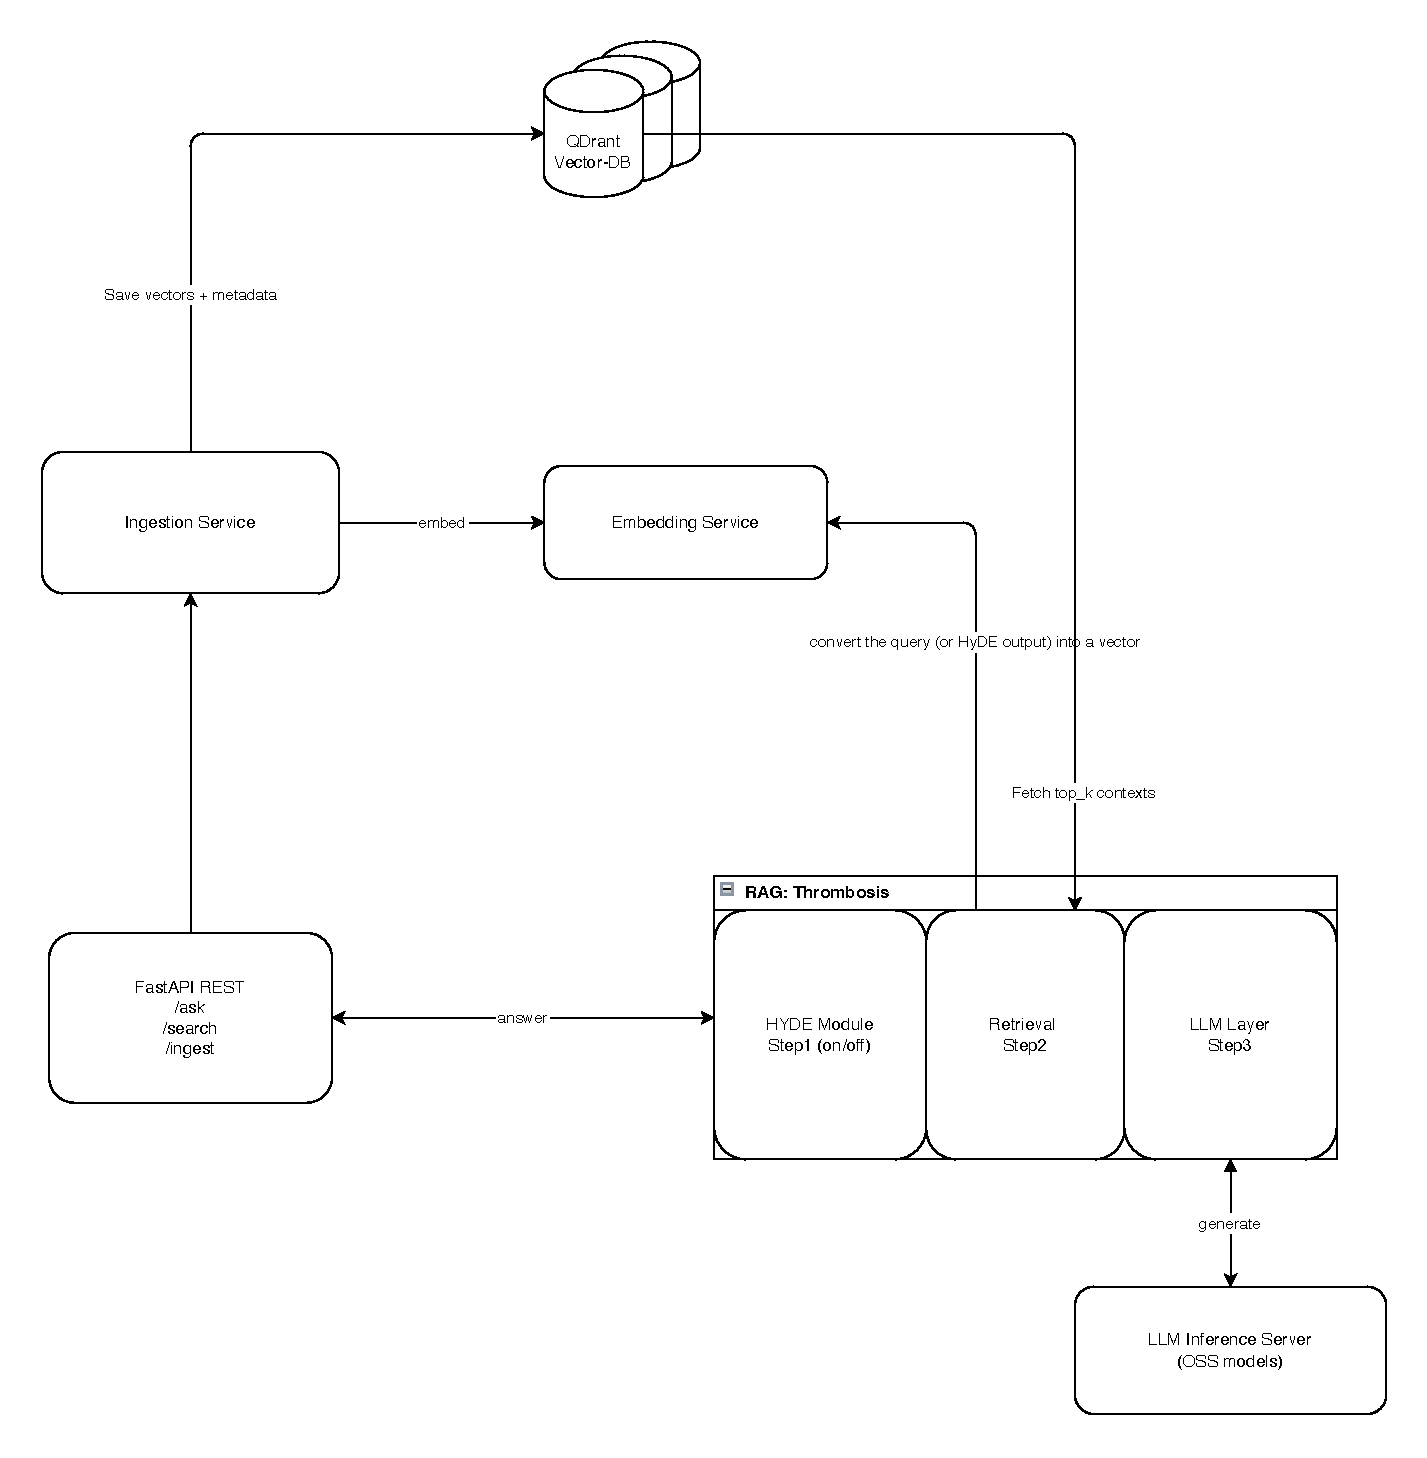
\includegraphics[width=\linewidth,height=0.67\textheight,keepaspectratio]{HLD.pdf}
\end{column}
\end{columns}
\end{frame}

\begin{frame}{RAG Pipeline}
\begin{itemize}
  \item Curated abstracts or scheduler-discovered PubMed records enter the ingestion API.
  \item Documents are split into section-aware chunks and embedded with a local sentence-transformer model.
  \item Qdrant stores vectors with DOI-centered metadata for traceable retrieval and deletion.
  \item Query-time retrieval creates a bounded evidence context before answer synthesis.
  \item Generated answers are constrained to structured JSON with citations to retrieved chunks.
\end{itemize}
\end{frame}

\begin{frame}{Data Ingestion and Indexing}
\begin{itemize}
  \item Documents can be introduced directly or through scheduler-initiated DOI and PMID workflows.
  \item Asynchronous ingestion jobs reserve document identities, enforce duplicate controls, and expose job status.
  \item Section-aware chunking filters non-informative text and retains bibliographic metadata.
  \item Indexing favors local reproducibility and traceability, while current queue and job state remain in memory.
\end{itemize}
\end{frame}

\begin{frame}{Retrieval and Generation}
\begin{itemize}
  \item Direct retrieval embeds the question and retrieves dense vector candidates from Qdrant.
  \item Optional HyDE generates a hypothetical passage and retrieves an additional candidate pool.
  \item Hybrid ranking combines dense rank, optional HyDE rank, BM25-style lexical signals, and section weights.
  \item Synthesis uses bounded context windows, strict JSON output, citation backfilling, and schema validation.
\end{itemize}
\end{frame}

\begin{frame}{Evaluation Overview}
\centering
\normalsize
\begin{tabular}{lccc}
\toprule
Configuration & Retrieval & Generation & Extraction \\
\midrule
LLM only & No & Yes & No \\
RAG & Yes & Yes & Yes \\
RAG + HyDE & Yes & Yes & Yes \\
\bottomrule
\end{tabular}

\vspace{0.45cm}
{\small Retrieval-dependent metrics apply only to the two RAG configurations. Numeric retrieval ranking metrics were not reported for the canonical run.}
\end{frame}

\begin{frame}{RAGAS Results Summary}
\centering
\small
\setlength{\tabcolsep}{5pt}
\begin{tabular}{lcccc}
\toprule
Configuration & Faithfulness & Answer Relevancy & Context Precision & Context Recall \\
\midrule
LLM only & \nr & 0.6104 & \nr & \nr \\
RAG + HyDE & 0.6458 & 0.8202 & 0.9000 & \nr \\
RAG & \textbf{0.8167} & \textbf{0.8672} & \textbf{1.0000} & \nr \\
\bottomrule
\end{tabular}

\vspace{0.3cm}
{\scriptsize Context recall was not reported in the canonical Chapter 7 run.}

\vspace{0.25cm}
\begin{block}{Takeaway}
RAG improved grounding relative to standalone generation. In this benchmark, RAG without HyDE delivered the strongest reported grounding scores.
\end{block}
\end{frame}

\begin{frame}{Extraction Results Summary}
\centering
\normalsize
\begin{tabular}{lccc}
\toprule
Configuration & Precision & Recall & F1 \\
\midrule
RAG + HyDE & \textbf{0.8350} & 0.9200 & 0.8735 \\
RAG & 0.8279 & \textbf{1.0000} & \textbf{0.9009} \\
\bottomrule
\end{tabular}

\vspace{0.35cm}
\begin{block}{Takeaway}
Risk factor extraction achieved high recall and strong F1 across both evaluated RAG configurations.
\end{block}
\end{frame}

\begin{frame}{Error Profile}
\centering
\normalsize
\begin{tabular}{lrrr}
\toprule
Configuration & TP & FP & FN \\
\midrule
RAG & 30 & 6 & 0 \\
RAG + HyDE & 29 & 5 & 2 \\
\bottomrule
\end{tabular}

\vspace{0.35cm}
\begin{block}{Takeaway}
\begin{itemize}
  \item RAG without HyDE produced zero false negatives.
  \item HyDE reduced false positives, but missed some reference factors.
  \item The preferred mode depends on whether sensitivity or specificity matters more.
\end{itemize}
\end{block}
\end{frame}

\begin{frame}{Operational Results}
\centering
\small
\begin{tabular}{lp{0.46\textwidth}}
\toprule
Metric & Value \\
\midrule
Questions & 5 thrombosis-oriented benchmark questions \\
Configurations & 3 answer-generation modes \\
Primary deterministic run & Seed 42, temperature 0.0 \\
Robustness condition & 5 stochastic seeds at temperature 0.2 \\
Extraction query coverage & 5/5 evaluated queries in both RAG modes \\
Recorded artifacts & Answers, RAGAS outputs, extraction summaries, diagnostics, configuration snapshots \\
\bottomrule
\end{tabular}
\end{frame}

\begin{frame}{Key Findings}
\begin{itemize}
  \item Retrieval was used in both RAG modes, but canonical ranking metrics such as nDCG, precision@k, and recall@k were not available for the reported run.
  \item RAG without HyDE achieved the strongest reported answer relevancy, faithfulness, and context precision.
  \item For extraction, RAG without HyDE achieved the best recall and F1, while HyDE achieved slightly higher precision.
  \item The evaluation pipeline was operationally auditable because it preserved configuration snapshots and phase-level outputs for deterministic and robustness runs.
  \item The main limitation is scope: only five benchmark questions and no canonical query-specific retrieval judgments.
  \item The clearest next step is a larger benchmark with explicit retrieval artifacts and judged relevance labels.
\end{itemize}
\end{frame}

\begin{frame}{Conclusion}
\begin{itemize}
  \item The thesis delivers an auditable local biomedical RAG platform rather than a standalone model demonstration.
  \item The architecture integrates PubMed acquisition, human curation, indexing, retrieval, cited synthesis, and evaluation.
  \item In the canonical benchmark, RAG without HyDE is the strongest overall configuration.
  \item The central contribution is a defensible engineering research foundation with explicit evidence, boundaries, and limitations.
\end{itemize}
\end{frame}

\end{document}
